\documentclass[12pt,a4paper]{article}
\usepackage[utf8]{inputenc}
\usepackage[russian]{babel}
\usepackage[OT1]{fontenc}
\usepackage{graphicx}
\usepackage{calc}
\usepackage[margin=15mm]{geometry}
% счётчик задач
\newcounter{notask}
\setcounter{notask}{1}

% условие без картинки
\newcommand{\task}[2]{
\hrule
\hbox to \textwidth {%
     \vrule
\parbox[t]{0.04\textwidth}{\smallskip \centering #1}%
     \vrule%
\hfill%
     \parbox[t]{0.93\textwidth}{\smallskip #2 \smallskip}\hfill%
\vrule
}
\hrule
    \addtocounter{notask}{1}
    \pagebreak[2]
}

\newlength{\h}
\newsavebox{\taskbox}
\newlength{\x}
\newsavebox{\pictbox}

% условие с картинкой (картинка выравнивается по центру)
\newcommand{\taskpic}[3]{
\savebox{\taskbox}{\parbox[t]{0.93\textwidth-4.3cm}{\smallskip #2 \smallskip}}
\savebox{\pictbox}{\parbox[t]{4cm}{\smallskip \centering
     \vspace{0pt} #3 \smallskip}}
\h=\ht\taskbox
\advance\h\dp\taskbox
\x=\ht\pictbox
\advance\x\dp\pictbox
\hrule
\hbox to \textwidth {%
\vrule\parbox[t][\maxof{\h}{\x}][t]{0.04\textwidth}{ \smallskip
     \centering #1 }\vrule%
\hfill\parbox[t][\maxof{\h}{\x}][t]{0.93\textwidth-4.3cm}{\smallskip #2
     \smallskip}\hfill\vrule%
\hfill\parbox[t][\maxof{\h}{\x}][c]{4cm}{\hfil #3 \hfil}\hfill\vrule
}
\hrule
\addtocounter{notask}{1}
\pagebreak[2]
}
\pagestyle{empty}
\graphicspath{ {images/} }

\begin{document}
\begin{center}
\begin{Large}
\textsc{ГЦФО. 9 класс. 2014/15.}
\end{Large}
\end{center}
\taskpic{5}{В солдата, сидящего в окопе, неприятель выстрелил из мортиры (см. рис.). Снаряд летел ровно на него, но до окопа не долетел. С точки зрения солдата снаряд поднимался в течение $t_1$ секунд, а опускался быстрее, за $t_2$ секунд, смотрел он из окопа от уровня земли. Известно, что неприятельские мортиры стреляют под углом $\alpha$ к горизонту, а модуль начальной скорости снаряда равен $V_0$. Найдите, на каком расстоянии от окопа упал снаряд. Сопротивлением воздуха пренебречь, ускорение свободного падения равно $g$.}{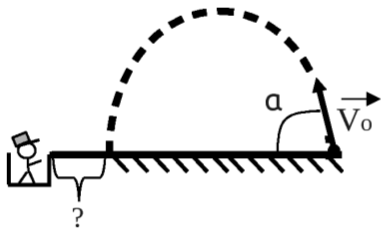
\includegraphics[width=4cm]{5}}
\taskpic{6}{Наклонная плоскость образует угол $\alpha$ с горизонтом. С высоты $H$ на нее падает мячик. Считая удары мячика о плоскость абсолютно упругими, определите расстояние между точками $n$-го и $(n+1)$-го отскока мячика от плоскости.}{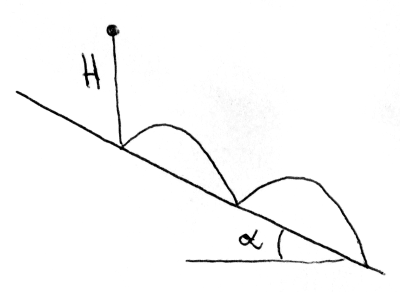
\includegraphics[width=3cm]{6}}
\taskpic{7}{Тело соскальзывает с гладкой горки с высоты $H$. Отрыв тела от горки происходит на высоте $h$, при этом скорость тела горизонтальна. При каком значении $h$ дальность полета тела будет максимальной?}{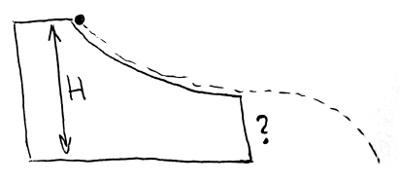
\includegraphics[width=4cm]{7}}
\taskpic{9}{Две прямые, пересекающиеся под углом $\alpha$, движутся перпендикулярно самим себе со скоростями $v_1$ и $v_2$.  Определите скорость $v$ точки пересечения прямых.}{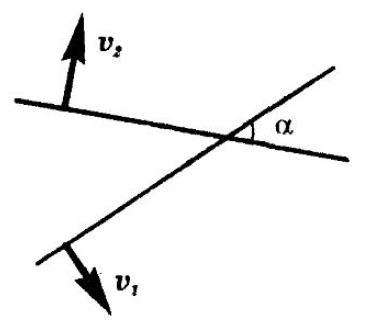
\includegraphics[width=3cm]{9}}
\taskpic{10}{Чиполлино решил сделать святящуюся эмблему своего любимого футбольного клуба <<Зенит>>. Он собрал электрическую схему, как показано на рисунке. Все буквы он составил из неоновых лампочек с одинаковым сопротивлением $R$ (на рисунке толстые черные линии между серыми точками) и соединил их проводами (сопротивление которых пренебрежимо мало, на рисунке тонкие линии). Лампа начинает светиться, если через нее течет сколь угодно малый ток. Нарисуйте, как выглядела светящаяся часть названия клуба, когда Чиполлино подключил напряжение к клеммам 1 и 2. Ответ поясните.}{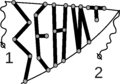
\includegraphics[width=4cm]{10}}
\task{11}{Два одинаковых вольтметра соединили параллельно, третий вольтметр подключили к этой комбинации последовательно, и к концам получившейся цепи присоединили идеальную батарейку. При этом вольтметры показывают 4 В, 4 В и 5 В. Какое напряжение у батарейки? Могут ли быть одинаковыми все три вольтметра? Что покажут эти же приборы, если их все соединить последовательно и подключить к той же батарейке? Показания приборов считайте точными.}

\end{document}